%!TEX root = ../EmbSW1.tex
\section{Concurrency}
\subsection{Introduction}
\subsubsection{Motivation}
Practical programs usually perform several jobs \glqq simultaneously\grqq.

\subsubsection{Definitions}
\begin{description}
	\item[Definition:] Concurrency refers to the ability of a system to process or execute processes independently of each other.
	      (Concurrency $\rightarrow$ Tasks/Processes $\rightarrow$ Threads)
	\item [Interrupt latency:] Refers to the interval of time from an external interrupt request signal being raised to the first ISR instruction being fetched and executed.
	\item [Interrupt response time:] Refers to the interval of time from an external IRQ signal being raised to the completion of the IRQ.
\end{description}
A key feature of embedded systems is the ubiquity of concurrency in applications.

\subsubsection{Parallel vs. Concurrent Computing}
\begin{itemize}
	\item Parallel Computing
	      \begin{itemize}
		      \item execution of different tasks is really at the same time
		      \item is not possible on a single-core machine
	      \end{itemize}
	\item Concurrent Computing
	      \begin{itemize}
		      \item execution of different tasks only seems to be at the same time
		      \item different tasks get consecutive time slices
		      \item there's only one task really running at a particular time slice
		      \item can be done on a single- or multicore machine
	      \end{itemize}
\end{itemize}

\subsubsection{Reasons to not use Concurrency}
\begin{itemize}
	\item \textbf{Concurrency (with Processes, Tasks, Threads) always cost}:
	      \begin{itemize}
		      \item Stack
		      \item Context switch
		            \begin{itemize}
			            \item takes time
			            \item Old context needs to be stored, new context needs to be loaded
		            \end{itemize}
		      \item Access to shared resources needs to be synchronized
		            \begin{itemize}
			            \item costs
			            \item prone to errors (is forgotten or done wrong)
		            \end{itemize}
	      \end{itemize}
	\item \textbf{Complexity increases}
	      \begin{itemize}
		      \item Sequential progams are easier to understand than parallel ones.
		      \item The goal should always be to keep a system as simple as possible.
	      \end{itemize}
\end{itemize}

\subsection{Causes of Interrupt Latency}
For most processor architectures, the processor usually completes the current instruction, which may be a multi-cycle instruction.
\begin{itemize}
	\item To save the current scene to restore the states when returning from the ISR, the processor pushes various necessary core registers (usually the program counter, flag registers, linker register, and so on) to the stack.
	\item Some processor architectures need additional software statements to select the right ISR.
	\item Time to fetch and decode the ISR instructions to fill the pipeline.
	\item Most memory systems that store the code (such as flash) usually have wait states because the memory system clock frequency is usually much slower than the CPU clock.
	\item The interrupt may be preempted by other higher-priority interrupts anytime, including before the first ISR instruction is executed.
\end{itemize}


\subsection{Interprocess Communication (IPC)}
In a multitasking system there may exist tasks that need to cooperate with each other by exchanging messages.
This is called intertask communication, which can be classified into two types:
\begin{description}
	\item[Synchronous:] The sender and receiver need to wait for each other until the message transmission is complete.
	\item[Asynchronous:] The sender may continue to execute its next instruction while the message is being delivered to the receiver.
\end{description}
Example of asynchronous intertask communication: message queues, pipes, sockets, and signaling.

\subsubsection{Pipes}
Pipes are simple message transfer mechanism.
Mostly used for communication between two objects.
\begin{itemize}
	\item A pipe is a container of unstructured bytes.
	\item A Pipe is a strictly FIFO buffer.
	\item A pipe is a kernel object that can be a named pipe or an unnamed pipe
\end{itemize}
\glqq{}Pipes\grqq provide a task-to-task, task-to-interrupt, and interrupt-to-task communication mechanism.
However, the features of Pipes depend on the technology used.

\paragraph{Usage Patterns}
\columnratio{0.6}
\begin{paracol}{2}
	\textbf{Unidirectional Communication:} Task A writes and task B reads from pipe.
	The pipe delivers everything to manage the data flow (full, empty, data available).
	\switchcolumn
	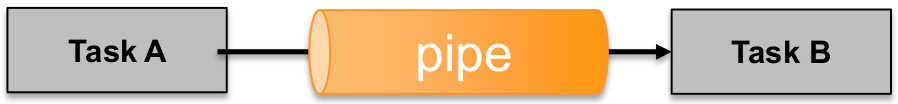
\includegraphics[width=0.39\textwidth]{images/Concurrency/uni_pipe.png}
	\switchcolumn
	\textbf{Bidrectional Communication:} Two pipes are needed to realize this pattern.
	\switchcolumn
	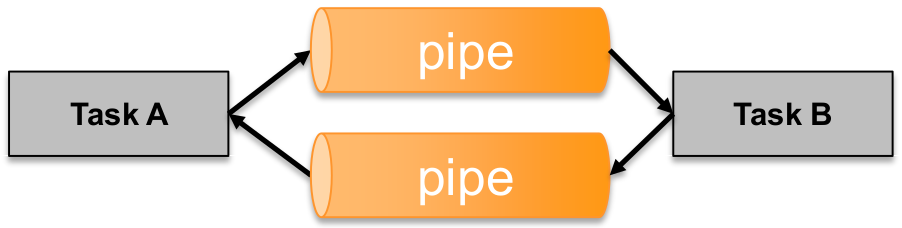
\includegraphics[width=0.39\textwidth]{images/Concurrency/bi_pipe.png}
\end{paracol}

\subsubsection{Queues}
Queues are an underlying mechanism beyond all tasks communication or synchronization in an operating system.
They are an important subject to understand as it is unavoidable to be able to build a complex application with tasks cooperating with each other.
They are a mean to store a and finite number (named \glqq{}length\grqq) of fixed size data.
They are able to be read and written by several different tasks, and don't belong to any task in particular.
A queue is normally a FIFO which means elements are read in the order they have been written.
This behavior depends on the writing method: two writing functions can be used to write either at the beginning or at the end of this queue.
\begin{itemize}
	\item A message queue is a container of multiple messages, each of which can be manipulated by a task separately.
	\item Each message in a message queue is associated with a priority; consequently, messages can be processed by tasks in priority order.
	\item A message queue is a named kernel object, with a name uniquely defined in the kernel’s namespace.
\end{itemize}
\glqq{}Queues\grqq provide a task-to-task, task-to-interrupt, and interrupt-to-task communication mechanism.
However, the features of Queues depend on the technology used (FreeRTOS supports less features).

\paragraph{Usage Patterns}
\columnratio{0.6}
\begin{paracol}{2}
	\textbf{Unidirectional Communication:} Task A writes and task B reads from queue.
	The queue delivers everything to manage the data flow (full, empty, data available).
	\switchcolumn
	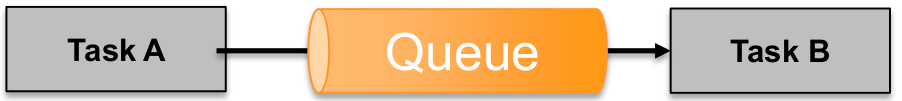
\includegraphics[width=0.39\textwidth]{images/Concurrency/uni_queue.png}
	\switchcolumn
	\textbf{Acknowledged Unidirectional Communication:}
	Similar approach as unidirectional communication, except that there is a semaphore used to signal that data was successfully received.
	Otherwise, a repetition can be triggered by task A.
	\switchcolumn
	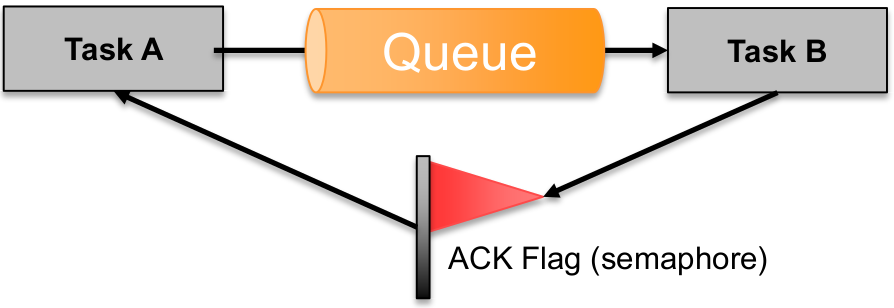
\includegraphics[width=0.39\textwidth]{images/Concurrency/ack_queue.png}
	\switchcolumn
	\textbf{Bidrectional Communication:} Two queues are needed to realize this pattern.
	\switchcolumn
	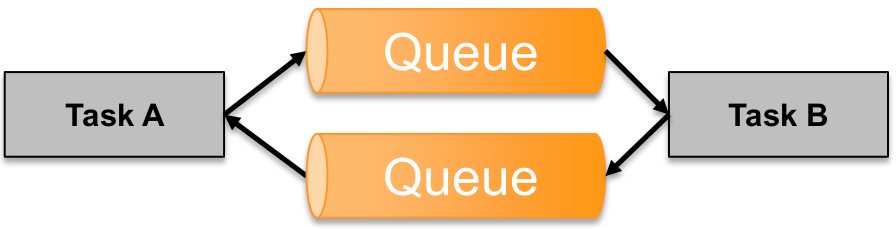
\includegraphics[width=0.39\textwidth]{images/Concurrency/bi_queue.png}
\end{paracol}


\subsection{Resource Sharing}
\subsubsection{Definitions}
\begin{description}
	\item[Race Condition]  The result of an operation depends on the timing behaviour of a specific operation.
	\item[Starvation]      Is a condition where a process never gets to it (it starves).
	      The fairness condition states that starvation must be prevented.
	\item[Deadlock]        Is a situation where two processes block each other.
	      A deadlock can be avoided by having all processes request the shared resources always in the same order.
	\item[Shared Variable] If the variable is accessible by all process, then the access is easy to establish.
	      However race conditions can occur and data integrity is an issue.
	\item[Shared Memory] An object (a regular file or memory object) can be directly mapped into the address space of one or more processes.
	      Memory mapping makes the mapped region of the object directly addressable by a process.
	      This eliminates unnecessary data read, write, or copy operations, and thus offers an efficient means of passing data between processes running on the same machine.
	      However shared memory is also a shared resource.
	      Therefore, Resource management mechanism must be used for usage of the shared memory.
	      Depending on the used technology (OS, language architecture) these mechanism are included in the shared memory object.
	\item[Priority Inversion] POSIX-compliant RTOSs implement a priority-based preemptive scheduler, which ensures that among all the threads that are ready to run, the one with the highest priority is always the task that is actually running.
	      When a higher-priority thread is released, the scheduler will preempt the currently running thread in the middle of its execution.
	      However, priority-based preemptive scheduling could be compromised when tasks share exclusive resources that are protected by locks:
	      Requesting a resource locked by a lower-priority task would prevent a higher-priority ready task from running when it should.
	      This issue is called priority inversion, referring to the phenomenon where a higher-priority task must wait for the lower-priority task.
	      Priority inversion is a critical issue because it may lead to the missing of task deadlines.
\end{description}
Shared memory support:
\begin{description}
	\item[Linux, Mac, Windows:] Support shared memory in the IDEs
	\item[OpenMP:] Software library for C and C++ delivers also support for shared memory
	\item[FreeRTOS:] No explicit support of shared memory
	\item[CMSIS RTOS2:] Example to implement a shared memory: \href{https://arm-software.github.io/CMSIS_5/RTOS2/html/rtos_api2.html}{MemoryPool}
\end{description}

\subsubsection{Prevention}
\paragraph{Race Conditions}
\begin{description}
	\item[Critical Sections] Define sections in which ISR(s) are blocked.
	      Pro: Simple, possible on any MCU.
	      Cons: Acts blocking.
	\item[Atomic Operations] Command disables ISR for one instruction cycle.
	      Atomic commands can not be split in instruction cycles that can be interrupted.
	      Atomic by CPU architecture see RISC-V RV32A Atomic Extension.
	      Atomic by programming language.
	      \textbf{Atomic operation} is a \textbf{foundation} for all other solutions of OS and RTOS.
\end{description}

\paragraph{Deadlock}
\begin{enumerate}
	\item fixed sequence for all task on locking and unlocking the same resources.
	      Example: task A and B both first lock resource 1 and then resource 2
	\item Try with return.
	      Example tas A and B try to lock resource 2.
	      If resource 2 is already locked, then the tasks release resource 1
	\item Timed release.
	      Example: task A and B try to lock resource 2.
	      If resource 2 is not available after a defined time, then the task releases resource 1 again.
	\item Atomic or Critical Section
	      Example: taskk A and B lock resource 1 and resource 2 in an atomic manner or a critical section defined sequence.
\end{enumerate}

\paragraph{Priority Inversion}
\begin{description}
	\item[Priority inheritance Protocol (PIP):] When a low priority task is holding a resource and a higher priority task wants it.
	      Then the priority is inherited from the higher priority tas to the lower one.
	      Inheritance is also possible over several tasks, where the highest priority is inherited.
	\item[Highest Locker Protocol (HLP):] When a task takes a resource then its priority is dynamically set to the highest priority of the task pool which can take the resource.
	      (also kwnown as immediate priority inheritance, immediate ceiling priority or priority protect protocol)
	\item[Priority Ceiling Protocol (PCP):] Combines PIP and HLP.
	      When a low priority task is holding a resource and a higher priority task wants it then the priority is inherited from the highest priority of the task pool which can take the resource.
\end{description}

\subsubsection{Semaphores}
A semaphore an be used in various ways
\begin{itemize}
	\item Task synchronization (binary)
	\item Task ISR synchronization (binary)
	\item Counting events (counting)
	\item Flow control (share memory \& binary/counting)
	\item Resource management (binary/counting)
\end{itemize}

\paragraph{Binary Semaphore}
Binary semaphores are the simplest effective way to synchronize tasks, an other even more simple, but not as effective, consists in polling an input or a resource.
A binary semaphore can be seen as a queue which contains only one element.

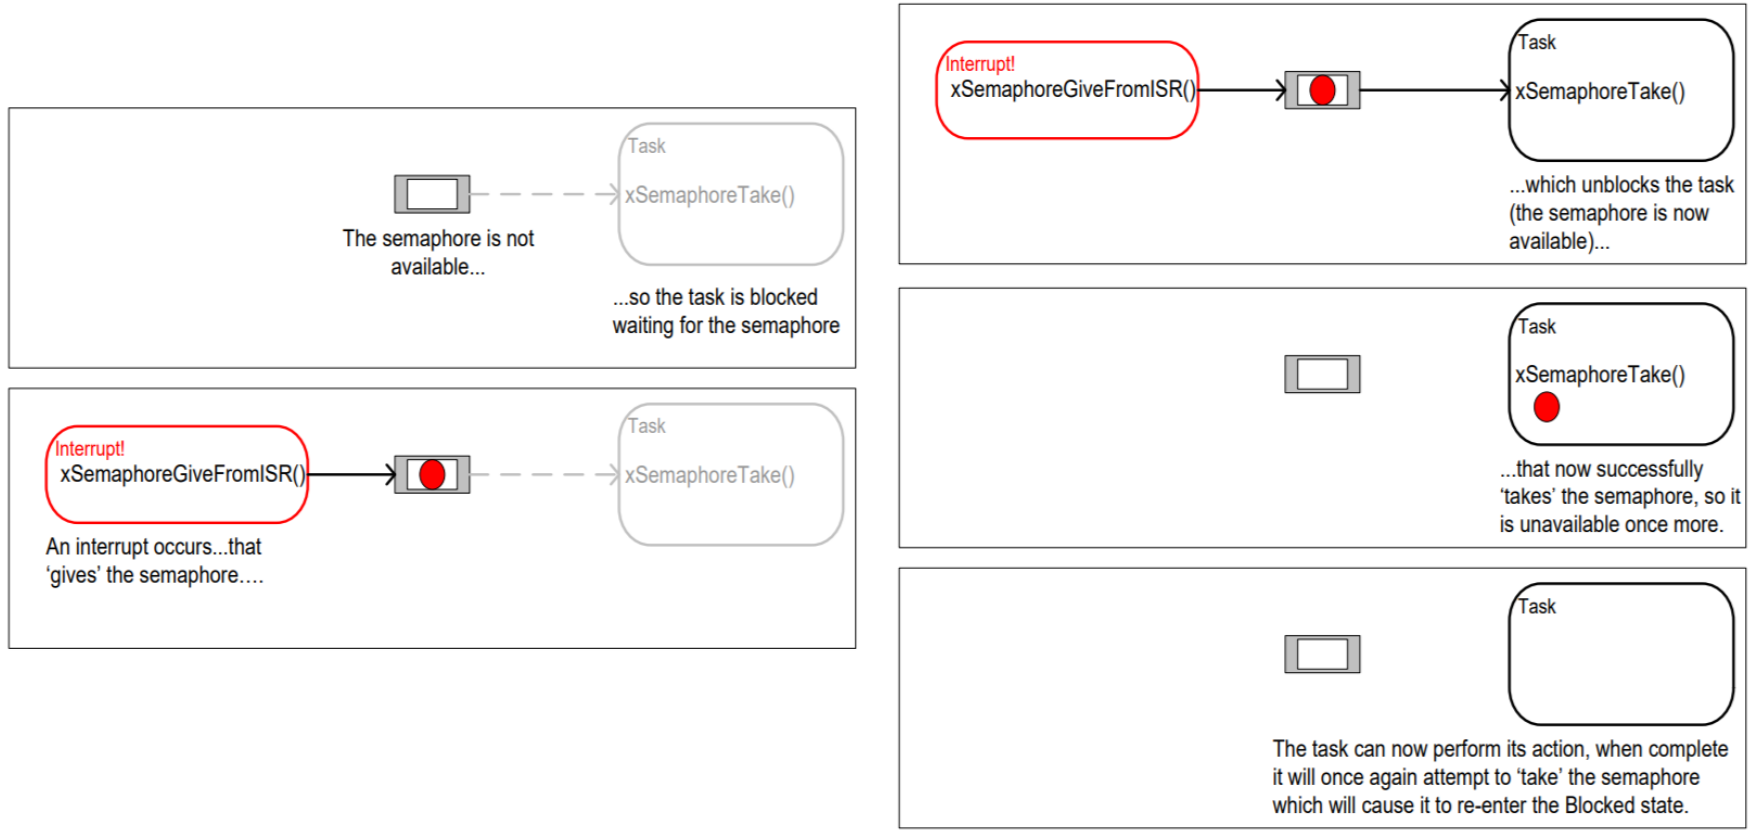
\includegraphics[width=\textwidth]{images/Concurrency/binary_semaphore.png}

\paragraph{Counting Semaphore}
A counting semaphore is a semaphore that can be taken several (but limited) times before it becomes unavailable.
It maintains a value which is increased as the semaphore is given, and decreased when it is taken.
Is is comparable to a queue with a certain amount of elements.
When created, a counting semaphore can be initialized to be available an arbitrary number of times.
The initial value and the maximum are defined on semaphore creation!

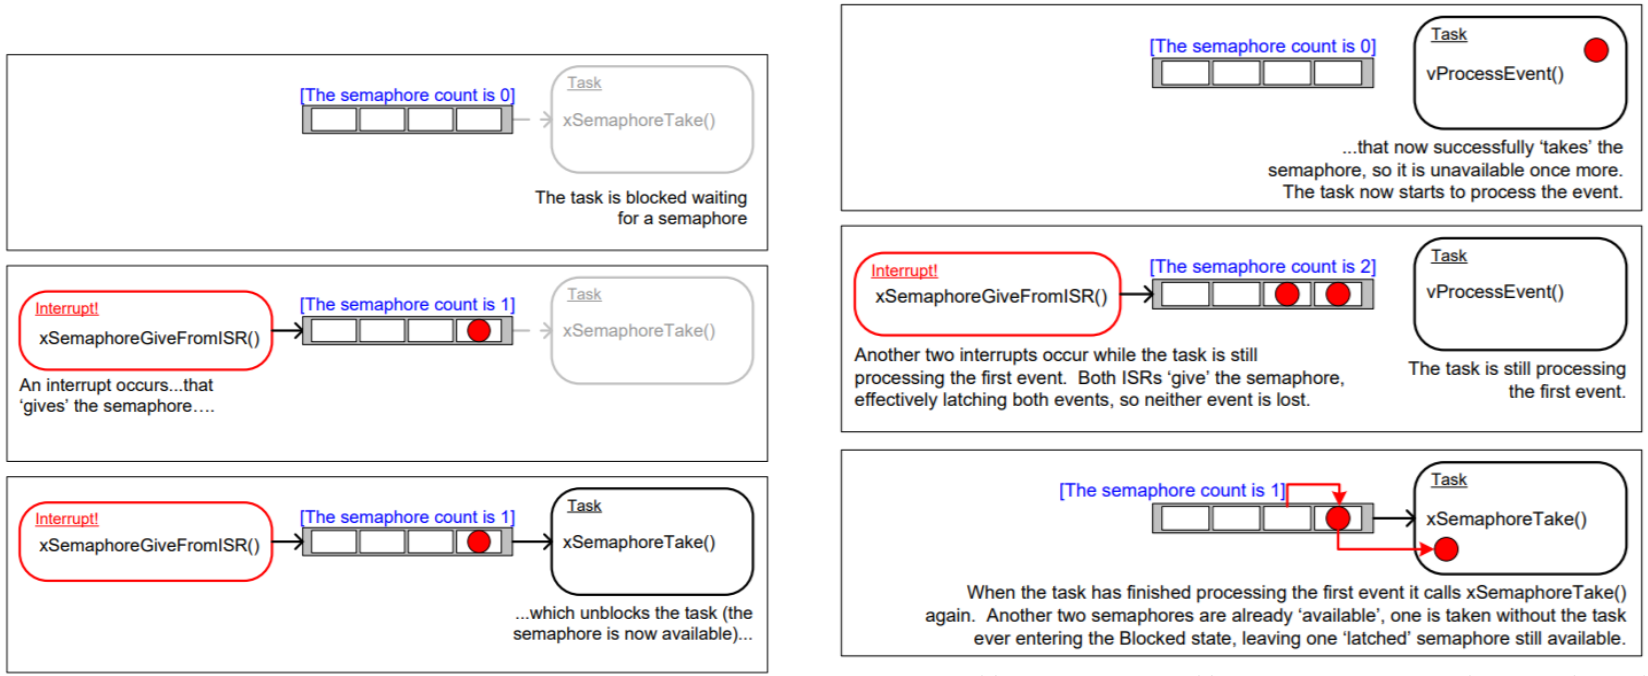
\includegraphics[width=\textwidth]{images/Concurrency/counting_semaphore.png}

\paragraph{Recommandations}
\begin{enumerate}
	\item Lock and release of Resources with semaphores costs time $\rightarrow$ less semaphores but bigger blocking regions
	\item If more tasks access semaphores, then blocking time gets longer.
	      More semaphores smaller blocking regions
	\item Approach 1 and 2 are counter rotating.
	      Case-specific decision, partly experimental
\end{enumerate}
In principle, it is important to create minimum locking times in order to avoid unnecessary blocking time.

\subsubsection{Mutexes}
A mutex (= mutual exclusion) is used similarly to a binary semaphore, except the task which take the semaphore must give it back.
This can be though with a token associated with the resource to access to.
A task holds the token, works with the resource then gives back the token; in the meanwhile, no other token can be given to the mutex.
Mutexes are mostly implemented blocking.

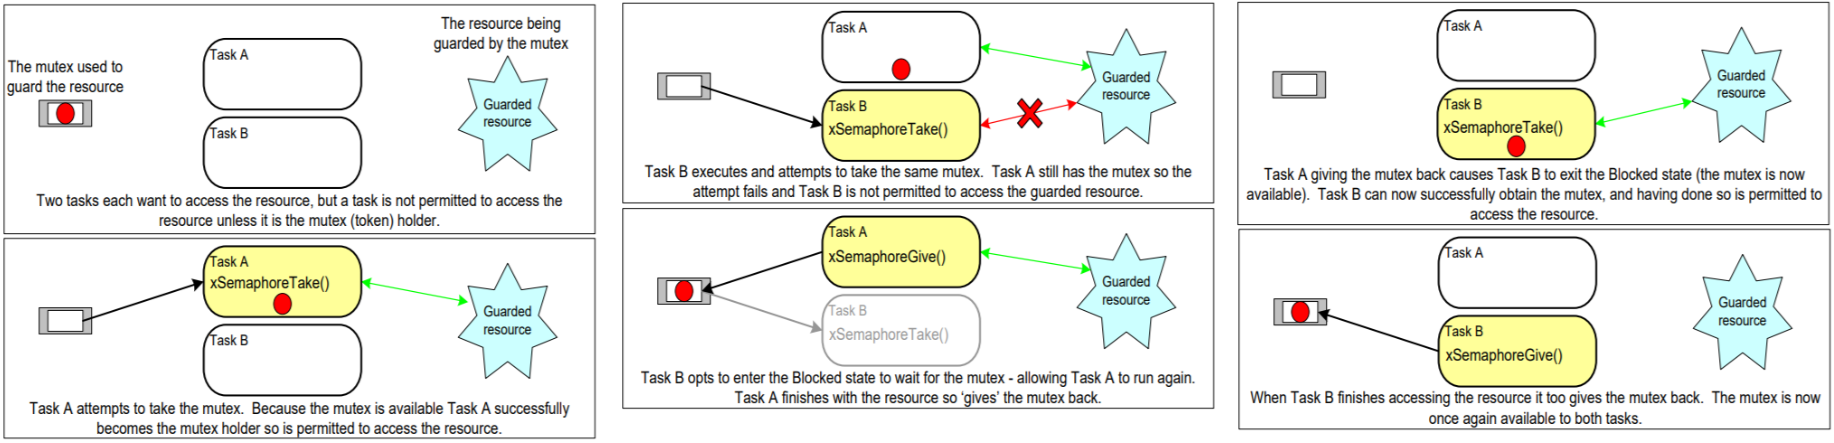
\includegraphics[width=\textwidth]{images/Concurrency/mutex.png}

\subsubsection{Recursive Mutex}
The issue arises when a task several times locks the mutex.
Consequently, it will also several time unlock the mutex.
If locking can only be done once all following locks are not counted.
If a unlock command arises the the mutex is released even if a task logic has locked it for it.

Solution:
Every lock of the mutex is counted and must be unlocked to release the mutex.
A recursive Mutex is a counting Mutex!


\subsection{Function Reentrancy}
In an RTOS the function should be thread safe:
A function is \glqq{}reentrant\grqq{} or thread safe if it is safe to call the function from more than one task, or from both tasks and interrupts.
Reentrant functions are said to be \glqq{}thread safe\grqq{} because they can be accessed from more than one thread of execution without the risk of data or logical operations becoming corrupted.
Each task maintains its own stack and its own set of processor (hardware) register values.
If a function does not access any data other than data stored on the stack or held in a register, then the function is reentrant, and thread safe.

That's also a reason why there are different implementations of functions for ISR and tasks.
% \textbf{Folgerung:} Concurrency nur dann einsetzen, wenn wirklich ein Nutzen vorhanden ist!\\
% Tendenziell werden speziell bei Verwendung eines RTOS zu viele Threads definiert, welche das System nur komplexer und komplizierter machen $\rightarrow$ \textbf{Sequential} is simple, \textbf{concurrent} is error-prone

% \subsection{POSIX Threads Programming}
% \subsubsection{UNIX Process}
% \begin{itemize}
%   \item Heavyweight process (created by the operating system)
%   \item Processes require a fair amount of overhead; they contain information about program resources and program execution state, including: Process ID, process group ID, user ID, and group ID; Environment; Program instructions; Registers; Stack; Heap; File descriptors; Signal actions; Shared libraries; Inter-process communication tools
% \end{itemize}

% \subsubsection{UNIX Thread}
% \begin{itemize}
%   \item Lightweight "'process"'
%   \item \textbf{Threads use and exist within the process resources}
%   \item \textbf{A thread uses the same address space as other threads of the same process}
%   \item Threads are able to be scheduled by the operating system
%   \item Independent stream of instructions that may run simultaneously to other streams of instructions
%   \item Procedure that runs independently from its main program
%   \item A thread maintains its own: Stack pointer; Registers; Scheduling properties; Set of pending and blocked signals; Thread specific data
%   \item Concurrent programs are usually achieved with threads
% \end{itemize}

% \subsubsection{Process vs. Thread in UNIX}
% 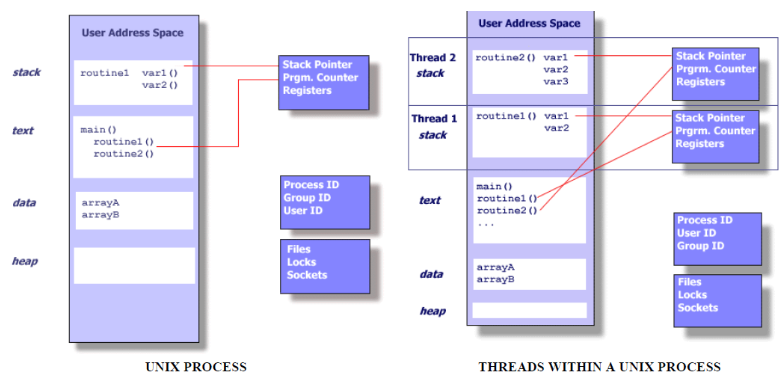
\includegraphics[width=12cm]{images/Concurrency/ProcessVsThread.png}\\\\
% Man beachte: Alles was ein Thread inne hat, hat ein Prozess auch inne (aber NICHT umgekehrt)!

% \subsection{What are POSIX Threads?}
% \begin{itemize}
%   \item For UNIX systems, a standardized C language threads programming interface has been specified by the \textbf{IEEE POSIX 1003.1c standard}.
%   \item The short form of \textbf{POSIX threads} is \textbf{Pthreads} or \textbf{pthreads}.
%   \item When compared to the cost of creating and managing a process, a thread can be created with much less operating system overhead
%   \item Managing threads requires fewer system resources than managing processes
% \end{itemize}

% \subsubsection{The pthreads API}
% \begin{itemize}
%   \item Routines of the pthreads API start with \textbf{pthread\_}
%   \item The header file \textbf{pthread.h} must be included
%   \item Source files that use pthreads shall be compiled and linked with \textbf{-pthread}
%   \item The link command must include \textbf{–lpthread}
% \end{itemize}

% \subsubsection{Starting and Terminating a Thread}
% \begin{itemize}[noitemsep,topsep=0pt]
%   \item Any routine with the following interface may become a thread routine: \lstinline{void* threadRoutine(void* arg);}
%   \item A thread is started with:\newline
%         \lstinline{int pthread_create(pthread_t* thread, const pthread_attr_t* attr, void* (*startRoutine) (void*), void* arg);}
%         \begin{itemize}[noitemsep,topsep=0pt]
%           \item thread: pointer to a pthread\_t instance
%           \item attr: pointer to a pthread\_attr\_t structure, often 0 (default attributes)
%           \item arg: a single argument that may be passed to startRoutine
%           \item returns 0 on success
%         \end{itemize}
%   \item A thread terminates in one of the following ways:
%         \begin{itemize}[noitemsep,topsep=0pt]
%           \item it calls pthread\_exit()
%           \item it returns from startRoutine
%           \item it is canceled with pthread\_cancel()
%         \end{itemize}
% \end{itemize}

% \textbf{Example - Starting a Thread}
% \begin{lstlisting}[style=C, escapechar=!]
% #include <pthread.h>
% void* threadFunction(void* arg);
% int main(void)
% {
%   pthread_t myT; !\tikz[remember picture] \node [] (a) {};!
%   int ret = pthread_create!\tikz[remember picture] \node [] (b) {};!(&myT, 0, threadFunction, 0);
%   if (ret)
%   {  // handle error
%     return -1;
%   }
%   while (1) {} // endless loop
%   pthread_exit(0);
% }
% void* threadFunction(void* arg)
% {  // implement this
%   pthread_exit(0);
% }
% \end{lstlisting}
% \begin{tikzpicture}[remember picture, overlay,
%     every edge/.append style = { ->, thick, >=stealth, dashed, line width = 1pt},
%     every node/.append style = { align = left, minimum height = 10pt, font = \bfseries, fill= green!20},
%     text width = 5.5cm]
%   \node [right=8cm of a] (A) {myT becomes the reference to the thread};
%   \node [below right=.5cm and 3cm of b, text width=8.5cm] (B) {starts thread and immediately returns (thread may not yet be fully started)};
%   \draw (A.west) edge (a.east);
%   \draw[->, to path={-| (\tikztotarget)}] (B.west) edge (b.south);
% \end{tikzpicture}

% \textbf{Example - Waiting on a Thread to Finish}
% \begin{lstlisting}[style=C, escapechar=!]
% #include <pthread.h>
% void* threadFunction(void* arg);
% int main(void)
% {
%   pthread_t myT;
%   pthread_attr_t attr;
%   pthread_attr_init(&attr); // initialize and set thread detached attribute
%   pthread_attr_setdetachstate(&attr, PTHREAD_CREATE_JOINABLE);
%   int ret = pthread_create(&myT, &attr, threadFunction, 0); // only starts and returns
%   if (ret)
%   {  // handle error
%     return -1;
%   }
%   pthread_attr_destroy(&attr); // free attribute
%   ret = pthread_join(myT, 0);!\tikz[remember picture] \node [] (a) {};!
%   if (ret)
%   {  // handle error
%     return -1;
%   }
%   pthread_exit(0);
% }
% void* threadFunction(void* arg)
% {  // implement this
%   pthread_exit(0);
% }
% \end{lstlisting}
% \begin{tikzpicture}[remember picture, overlay,
%     every edge/.append style = { ->, thick, >=stealth, dashed, line width = 1pt},
%     every node/.append style = { align = left, minimum height = 10pt, font = \bfseries, fill= green!20},
%     text width = 7.5cm]
%   \node [right=5cm of a] (A) {main thread waits on myT to finish};
%   \draw (A.west) edge (a.east);
% \end{tikzpicture}
% %\lstinputlisting[style=C]{snippets/Threads/thread_waiting.c}

% \subsubsection{Thread-safeness}
% \begin{itemize}
%   \item Thread-Sicherheit besagt, dass eine Komponente gleichzeitig von verschiedenen Programmbereichen mehrfach ausgeführt werden kann, ohne dass diese sich gegenseitig behindern.
%   \item Änderungen der einzelnen Threads müssen koordiniert werden, um einen chaotischen Zustand des Speichers zu verhindern, da das Programm dabei häufig gleichzeitig auf einen gemeinsamen Speicherbereich (Shared Memory) des Computers zugreifen will.
%   \item Vorsicht: rand() ist nicht thread-safe (weil bei dieser Fkt. eine interne Variable verwendet wird, welche schon zum Voraus berechnet wurde); rand\_r() hingegen schon.
% \end{itemize}

% \subsubsection{Quasiparallelität und "'Prozess"'-Zustände}
% \begin{minipage}[c]{8cm}
%   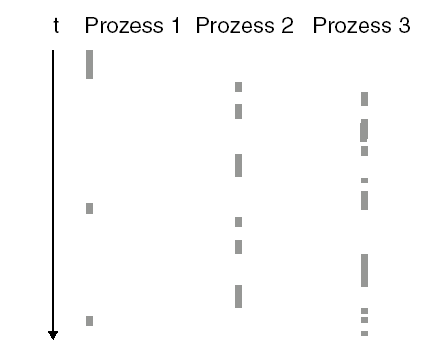
\includegraphics[width=5cm]{images/Concurrency/Quasiparallelitaet.png}
% \end{minipage}
% \begin{minipage}[c]{10cm}
%   \begin{itemize}
%     \item Prozesse/Threads warten die meiste Zeit (blocked).
%     \item Scheduler ordnet CPU denjenigen Prozessen/Threads zu, die im Zustand ready sind und "'etwas zu tun haben"'
%   \end{itemize}
% \end{minipage}\\\\
% Prozesse/Threads können folgende Zustände und Übergänge erfahren:\\
% \begin{minipage}[c]{8cm}
%   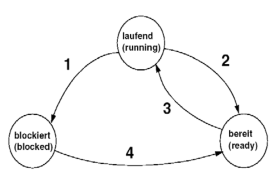
\includegraphics[width=6cm]{images/Concurrency/Prozesszustaende.png}
% \end{minipage}
% \begin{minipage}[c]{10cm}
%   \begin{enumerate}
%     \item I/O Operation, Warten auf Bedingung
%     \item Scheduler entzieht CPU
%     \item Scheduler weist CPU zu
%     \item I/O beendet, Bedingung erfüllt
%   \end{enumerate}
% \end{minipage}

% \subsection{Synchronisation: Zugriff auf gemeinsame Ressourcen}
% \subsubsection{Kritischer Abschnitt (Critical Section, CS)}
% \begin{itemize}
%   \item Codebereich, in dem nebenläufige oder parallele Prozesse auf gemeinsame Ressourcen zugreifen. Zu jeder Zeit darf sich höchstens ein Prozess im kritischen Bereich
%         befinden.
%   \item Der exklusive Zugriff durch höchstens einen Prozess wird mittels gegenseitigem Ausschluss (mutual exclusion, Mutex) sichergestellt.
% \end{itemize}

% \subsubsection{Lösungsstruktur für gegenseitigen Ausschluss}
% \begin{minipage}[c]{2cm}
%   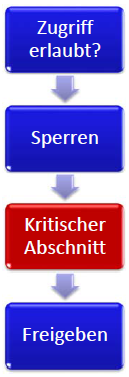
\includegraphics[width=1.5cm]{images/Concurrency/Loesungsstruktur.png}
% \end{minipage}
% \begin{minipage}[c]{14cm}
%   \begin{itemize}
%     \item Bei der Zugriffsprüfung wird gewartet, bis der Zugang frei wird \\ \ \\
%     \item Beim Sperren wird das Signal auf Rot gesetzt (lock a mutex) \\ \ \\
%     \item Beim Freigeben wird das rote Signal wieder gelöscht (unlock a mutex)
%   \end{itemize}
% \end{minipage}

% \subsubsection{Forderungen an die Synchronisation (Dijkstra, 1965)}
% \begin{enumerate}
%   \item Es dürfen sich nicht zwei Prozesse gleichzeitig in ihrem kritischen Abschnitt befinden (mutual exclusion).
%   \item Über die Abarbeitungsgeschwindigkeit, bzw. die Anzahl Prozesse dürfen keine Annahmen getroffen werden.
%   \item Kein Prozess darf ausserhalb eines kritischen Abschnitts einen anderen Prozess blockieren.
%   \item Jeder Prozess, der am Eingang eines kritischen Abschnitts wartet, muss irgendwann den Abschnitt betreten dürfen (fairness condition).
% \end{enumerate}

% % \begin{tabbing}
% %   \hspace*{1cm}\=\hspace*{4.2cm}\=\hspace*{3cm}\=\hspace*{2.7cm}\= \kill
% % \textbf{Synchro-Versuch 1}\\\\
% %   \>{\textbf Prozess 1} \> \> \>{\textbf Prozess 2}\\
% %   \>\begin{lstlisting}[style=C]
% % while(grant != 1)
% %     wait();
% % CS; //Eintritt in Critical Section
% % grant = 2;
% %     \end{lstlisting} \> \> \>
% %     \begin{lstlisting}[style=C]
% % while(grant != 2)
% %     wait();
% % CS; //Eintritt in Critical Section
% % grant = 1;
% %     \end{lstlisting} \\\\
% %     Forderung 2 nicht erfüllt, da sich alle Prozesse selbst daran hindern 2mal nacheinander daran zu kommen.\\\\
% %
% % \textbf{Synchro-Versuch 2}\\\\
% %    \>{\textbf Prozess 1} \> \> \>{\textbf Prozess 2}\\
% %    \>\begin{lstlisting}[style=C]
% % while(in2)
% %     wait();
% % in1 = true;
% % CS; //Eintritt in Critical Section
% % in1 = false;
% %     \end{lstlisting} \> \> \>
% %     \begin{lstlisting}[style=C]
% % while(in1)
% %     wait();
% % in2 = true;
% % CS; //Eintritt in Critical Section
% % in2 = false;
% %     \end{lstlisting} \\\\
% %     Initialisierung ist nicht gelöst.\\\\
% %
% % \textbf{Synchro-Versuch 3 (Algorithmus von Peterson)}\\\\
% %    \>{\textbf Prozess 1} \> \> \>{\textbf Prozess 2}\\
% %    \>\begin{lstlisting}[style=C]
% %         request1 = true;
% %         grant = 1;
% %         while(grant==1 && request2)
% %           wait();
% %         CS; //Eintritt in Critical Section
% %         request1 = false;
% %     \end{lstlisting} \> \> \>
% %     \begin{lstlisting}[style=C]
% %         request2 = true;
% %         grant = 2;
% %         while(grant==2 && request1)
% %           wait();
% %         CS;  //Eintritt in Critical Section
% %         request2 = false;
% %     \end{lstlisting} \\
% % \end{tabbing}
% % \vspace*{-1cm}

% \subsubsection{Synchronisation mit Signalen}
% \begin{itemize}
%   \item Jeder Prozess wartet vor Betreten des kritischen Bereichs auf ein
%         gemeinsames Signal.
%   \item Wenn Signal gesetzt $\rightarrow$ kritischer Bereich frei
%   \item waitfor(signal) blockiert aufrufenden Prozess, falls signal nicht
%         gesetzt
%   \item Jeder Prozess, der fertig ist, setzt Signal mit send(signal)
%   \item Mehrere Prozesse können gleichzeitig warten
%   \item Es ist Aufgabe des Schedulingalgorithmus' bei gesetztem Signal einem der wartenden Prozesse das Betreten des kritischen Abschnitts zu gewähren
% \end{itemize}

% \begin{tabbing}
%   \hspace*{1cm}\=\hspace*{4.2cm}\=\hspace*{3cm}\=\hspace*{2.7cm}\= \kill
%   \>{\textbf Prozess 1} \> \> \>{\textbf Prozess 2}\\
%   \>\begin{lstlisting}[style=C]
% waitFor(signal);
% CS;  //Eintritt in Critical Section
% send(signal);
%     \end{lstlisting} \> \> \>
%   \begin{lstlisting}[style=C]
% waitFor(signal);
% CS;  //Eintritt in Critical Section
% send(signal);
%     \end{lstlisting} \\\\
% \end{tabbing}
% \vspace*{-1.5cm}

% \subsection{Semaphoren}
% \begin{itemize}
%   \item Das Signal für den Zutritt in den kritischen Bereich = Semaphor
%   \item Ein Semaphor s hat zwei atomare (= nicht unterbrechbare)
%         Operationen
%         \begin{itemize}
%           \item P(s) : Passieren $\rightarrow$ Beim Eintritt in CS (waitFor)
%           \item V(s) : Verlassen $\rightarrow$ Beim Austritt aus CS (send)
%         \end{itemize}
%   \item Busy waiting
%         \begin{itemize}
%           \item Beim Busy Waiting warten die Prozesse aktiv in einer Schleife (spin lock)
%           \item Wartende Prozesse belasten so unnötigerweise den Prozessor
%           \item \textbf{Lösung:} Wartende Prozesse werden in eine Warteschlange eingetragen (sleep und
%                 wakeup)
%         \end{itemize}
%   \item Probleme der Semaphoren
%         \begin{itemize}
%           \item Anwendung erfordert viel Disziplin
%                 \begin{itemize}
%                   \item Für jedes P(s) braucht es auch ein V(s)
%                   \item Probleme treten auf, wenn V(s) vergessen geht! (Ressource bleibt besetzt)
%                 \end{itemize}
%           \item In grösseren Programmen können subtile Probleme entstehen, falls z.B. das V(s) in einer if-Bedingung gemacht wird.
%           \item Beim Auftreten einer Exception kann das Freigeben ebenfalls schwierig werden.
%         \end{itemize}
% \end{itemize}

% \subsection{Thread-Synchronisation in C mit POSIX Threads}
% \subsubsection{Mutual Exclusion (Mutex)}
% \begin{itemize}
%   \item A mutex variable acts like a "'lock"' protecting access to a shared data resource
%   \item The basic concept of a mutex as used in Pthreads is that only one thread can lock (or own) a mutex variable at any given time. Thus, even if several threads try to lock a mutex, only one thread will be successful.
%   \item No other thread can own that mutex until the owning thread unlocks that mutex
%   \item Very often the action performed by a thread owning a mutex is the updating of global (shared) variables
%   \item This is a safe way to ensure that when several threads update the same variable, the final value is the same as what it would be if only one thread performed the update
%   \item The variables being updated belong to a \textbf{critical section}
% \end{itemize}
% \textbf{A typical mutex sequence:}
% \begin{enumerate}
%   \item Create and initialize a mutex variable
%   \item Several threads attempt to lock the mutex
%   \item Only one succeeds and that thread owns the mutex
%   \item The owner thread performs some set of actions
%   \item The owner unlocks the mutex
%   \item Another thread acquires the mutex and repeats the process
%   \item Finally the mutex is destroyed
% \end{enumerate}

% \lstinputlisting[style=C]{snippets/Concurrency/Sync_POSIX.c}

% \subsubsection{Das Monitorprinzip}
% \begin{itemize}
%   \item Grundprinzip: Abstrakten Datenyp (ADT) definieren, der genau die Funktionen
%         in der Schnittstelle anbietet, die notwendig sind.
%   \item Der Aufrufer ruft diese Funktionen auf, er muss sich aber nicht um die
%         Synchronisation kümmern.
%   \item Die Synchronisation z.B. mit Semaphoren ist in der Implementation des
%         Monitors lokal gelöst.
%   \item Problem wird einmal im Monitor gelöst, die Aufrufer müssen sich nicht
%         mehr darum kümmern.
% \end{itemize}

% \subsubsection{Race condition/Starvation/Deadlock}
% \begin{description}
%   \item[Race Condition]  Das Ergebnis einer Operation hängt vom zeitlichen Verhalten bestimmter Einzeloperationen ab.
%   \item[Starvation]      Ist ein Zustand, bei dem ein Prozess nie dran kommt (er verhungert). Die Fairness condition besagt, dass Starvation verhindert werden muss.
%   \item[Deadlock]        Ist eine Situation in denen sich zwei Prozesse gegenseitig blockieren. Ein Deadlock kann vermieden werden, indem alle Prozesse die gemeinsamen Ressourcen immer in derselben Reihenfolge anfordern.
% \end{description}

% \subsection{Condition Variables}
% \begin{itemize}
%   \item Mutexes implement synchronization by controlling thread access to data
%   \item \textbf{Condition variables allow threads to synchronize based upon the actual value of data}
%   \item Without condition variables, the programmer would need to have threads continually polling (possibly in a critical section), to check if the condition is met
%   \item This can be very resource consuming since the thread would be continuously busy in this activity
%   \item \textbf{A condition variable is a way to achieve the same goal without polling}
%   \item A condition variable is always used in conjunction with a mutex lock
% \end{itemize}
% \begin{center}
%   \begin{minipage}{0.8\linewidth}
%     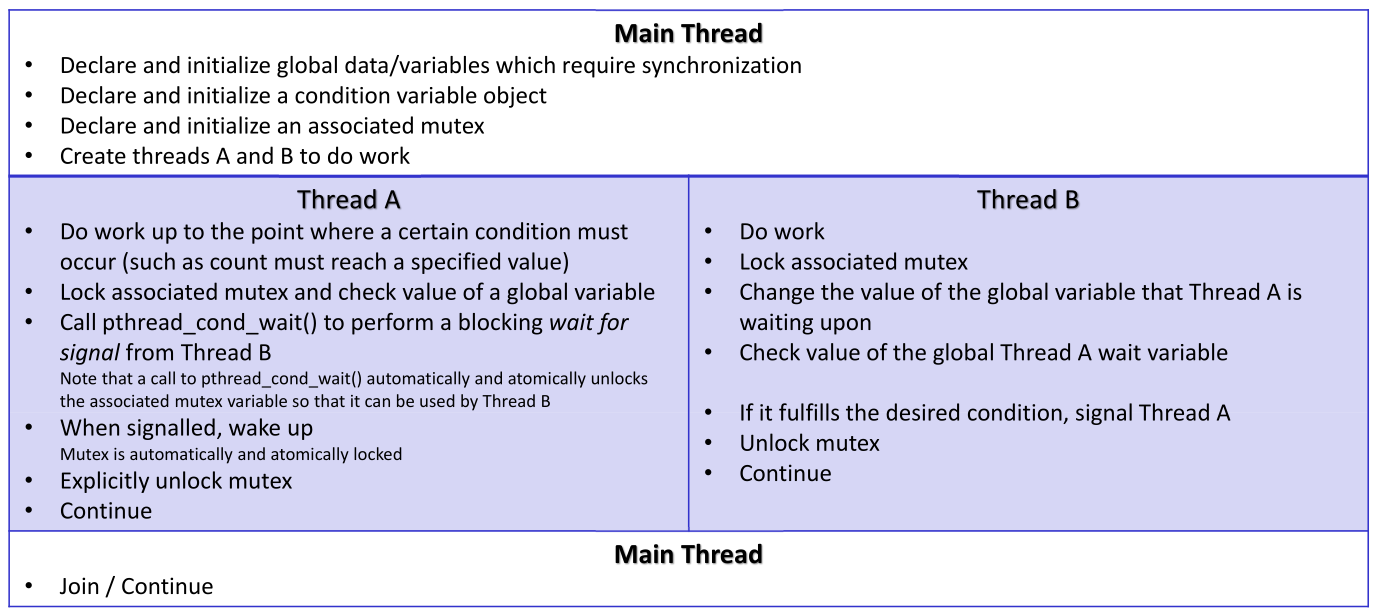
\includegraphics[width=\linewidth]{images/Concurrency/conditionVariablesAblauf}
%   \end{minipage}
% \end{center}

% \subsubsection{Creating and destroying condition variables}
% \begin{itemize}
%   \item Condition variables must be initialized before they can be used\newline
%         \lstinline{int pthread_cond_init(pthread_cond_t* condVar, const pthread_condattr_t* attr);}
%         \begin{itemize}
%           \item condVar: pointer to the condition variable
%           \item attr: pointer to a pthread\_condattr\_t structure, often 0 (default attributes)
%           \item returns 0 on success
%         \end{itemize}
%   \item The condition variables shall be destroyed when they're no longer needed\newline
%         \lstinline{int pthread_cond_destroy(pthread_cond_t* condVar);}
%         \begin{itemize}
%           \item condVar: pointer to the condition variable
%           \item returns 0 on success
%         \end{itemize}
% \end{itemize}

% \subsubsection{Waiting on condition variables}
% \begin{itemize}
%   \item waiting on condition variable: blocks calling thread until condition is signalled\newline
%         \lstinline{int pthread_cond_wait(pthread_cond_t* condVar, pthread_mutex_t* mutex);}
%         \begin{itemize}
%           \item condVar: pointer to the condition variable
%           \item mutex: pointer to the mutex
%           \item returns 0 on success
%         \end{itemize}
%   \item This routine should be called while mutex is locked
%   \item It will automatically release the mutex while it waits
%   \item After signal is received and thread is awakened, mutex will be automatically locked for use by the thread
%   \item The programmer is then responsible for unlocking mutex when the thread is finished with it
% \end{itemize}

% \subsubsection{Signaling on condition variables}
% \begin{itemize}
%   \item Signal on condition variable: unblocks thread blocked on a condition variable\newline
%         \lstinline{int pthread_cond_signal(pthread_cond_t* condVar);}
%         \begin{itemize}
%           \item condVar: pointer to the condition variable
%           \item returns 0 on success
%         \end{itemize}
%   \item This routine is used to signal (or wake up) another thread which is waiting on the condition variable
%   \item It should be called after mutex is locked, and must unlock mutex in order for pthread\_cond\_wait() routine to complete
% \end{itemize}

% \subsubsection{Using condition variables}
% \begin{itemize}
%   \item This example code demonstrates the use of several Pthread condition variable routines
%   \item The main routine creates three threads
%         \begin{itemize}
%           \item Two of the threads perform work and update a count variable
%           \item The third thread waits until the count variable reaches a specific value
%         \end{itemize}
%   \item The counting thread that reaches the specified count value signals (wakes up) the watching thread waiting on this condition
% \end{itemize}

% \lstinputlisting[style=C]{snippets/Concurrency/condVariableMain.c}
% \lstinputlisting[style=C]{snippets/Concurrency/condVariableIncCount.c}
% \lstinputlisting[style=C]{snippets/Concurrency/condVariableWatchCount.c}

% \subsubsection{Bounded Buffer Problem}
% \begin{itemize}[noitemsep,topsep=0pt]
%   \item The problem describes two processes, the producer and the consumer, who share a common, fixed-size buffer used as a queue.
%   \item The producer's job is to generate a piece of data, put it into the buffer and start again.
%   \item At the same time, the consumer is consuming the data (i.e., removing it from the buffer) one piece at a time.
%   \item The problem is to make sure that the producer won't try to add data into the buffer if it's full and that the consumer won't try to remove data from an empty buffer.
%   \item The problem can also be generalized to have multiple producers and consumers.
% \end{itemize}
% \textbf{Solution:}
% \begin{itemize}[noitemsep,topsep=0pt]
%   \item The solution for the producer is to either go to sleep or discard data if the buffer is full.
%   \item The next time the consumer removes an item from the buffer, it notifies the producer, who starts to fill the buffer again.
%   \item In the same way, the consumer can go to sleep if it finds the buffer to be empty.
%   \item The next time the producer puts data into the buffer, it wakes up the sleeping consumer.
%   \item The solution can be reached by means of inter-process/thread communication, typically using semaphores (mutexes).
%   \item An inadequate solution could result in a deadlock where both processes are waiting to be awakened.
% \end{itemize}

% \subsection{POSIX Interprocess Communication (IPC)}
% \begin{itemize}[noitemsep,topsep=0pt]
%   \item POSIX provides the following IPC mechanisms in the POSIX:XSI extension:
%         \begin{itemize}
%           \item Message queues in sys/msg.h
%           \item Semaphores in sys/sem.h
%           \item Shared Memory in sys/shm.h
%         \end{itemize}
%   \item These mechanisms allow unrelated processes to exchange information in a reasonably efficient way
% \end{itemize}

% \subsection{RAII (Resource Acquisition Is Initialisation)}
% \subsubsection{Motivation}
% \begin{itemize}[noitemsep,topsep=0pt]
%   \item Ressourcen (z.B. Datei, Speicher, etc.) müssen vor dem Gebrauch grundsätzlich angefordert werden
%   \item Nach Abschluss des Gebrauchs einer Ressource muss diese wieder freigegeben werden
%   \item Die saubere Anforderung und Freigabe ist fehlerträchtig
%   \item RAII löst diese Aufgabe elegant und zuverlässig
% \end{itemize}

% \subsubsection{Idee hinter RAII}
% \begin{itemize}[noitemsep,topsep=0pt]
%   \item Die Anforderung und Freigabe einer Ressource wird mit Hilfe einer Klasse implementiert:
%         \begin{itemize}
%           \item der Konstruktor fordert die Ressource an
%           \item der Destruktor gibt sie wieder frei
%         \end{itemize}
%   \item Die verwendete Ressource kann wie ein Objekt behandelt werden. Sobald das Objekt seine Gültigkeit verliert (z.B. out-of-scope), wird durch den Destruktor die Ressource "'automatisch"' freigegeben.
% \end{itemize}

% \subsubsection{Anwendung bei Heapobjekten}
% \begin{itemize}[noitemsep,topsep=0pt]
%   \item Wie kann man sicher gehen, dass ein Objekt, welches auf dem Heap angelegt wurde, auch wieder mittels delete sicher gelöscht wird?
%         \begin{itemize}
%           \item Exceptions können dazwischen kommen
%           \item C++03 kennt kein finally bei Exception-Handling
%         \end{itemize}
% \end{itemize}
% \begin{lstlisting}[style=C,escapechar=!]
% void f()
% {
%   Person* p = new Person("irgendwer");
%   // mach etwas mit p!\tikz[remember picture] \node [] (a) {};!
%   delete p;
% }
% \end{lstlisting}
% \begin{tikzpicture}[remember picture, overlay,
%     every edge/.append style = { ->, thick, >=stealth, dashed, line width = 1pt},
%     every node/.append style = { align = left, minimum height = 10pt, font = \bfseries, fill= green!20},
%     text width = 7.5cm]
%   \node [right=5cm of a] (A) {was ist, wenn hier eine Exception geworfen wird?};
%   \draw (A.west) edge (a.east);
% \end{tikzpicture}
% \textbf{Lösung:}
% \begin{itemize}[noitemsep,topsep=0pt]
%   \item Kapsle die dynamisch erzeugte Ressource mit einem Handle-Objekt auf dem Stack
%         \begin{itemize}[noitemsep,topsep=0pt]
%           \item Ideal std::shared\_ptr\textless T\textgreater aus Header \textless memory\textgreater
%         \end{itemize}
%   \item Der Destruktor dieses Handle-Objekts räumt beim Verlassen des Scopes automatisch auf. Das gilt auch für externe Ressourcen wie Files
% \end{itemize}
% \begin{lstlisting}[style=C,escapechar=!]
% #include <memory>
% void f()
% {
%   std::shared_ptr<Person> p(new Person("irgendwer"));
%   // mach etwas mit p
% }!\tikz[remember picture] \node [] (a) {};!
% \end{lstlisting}
% \begin{tikzpicture}[remember picture, overlay,
%     every edge/.append style = { ->, thick, >=stealth, dashed, line width = 1pt},
%     every node/.append style = { align = left, minimum height = 10pt, font = \bfseries, fill= green!20},
%     text width = 11cm]
%   \node [right=5cm of a] (A) {Beim Verlassen des Blocks räumt der Destruktor von shared\_ptr automatisch auf und löscht die Person};
%   \draw (A.west) edge (a.east);
% \end{tikzpicture}

% \subsubsection{Anwendung bei Mutex}
% \begin{itemize}[noitemsep,topsep=0pt]
%   \item Wie kann man sicher gehen, dass eine Mutex, die mit lock(m) angefordert wurde, in jedem Fall auch wieder mit unlock(m) freigegeben wurde?
%         \begin{itemize}
%           \item Exceptions können dazwischen kommen
%           \item Freigabe auch bei vorzeitigem Ausstieg mit return
%         \end{itemize}
% \end{itemize}
% \begin{lstlisting}[style=C,escapechar=!]
% static pthread_mutex_t m;
% // ...
% void f()
% {
%   pthread_mutex_lock(&m);
%   // mach etwas in kritischem Abschnitt!\tikz[remember picture] \node [] (a) {};!
%   pthread_mutex_unlock(&m);   // auf keinen Fall vergessen
% }
% \end{lstlisting}
% \begin{tikzpicture}[remember picture, overlay,
%     every edge/.append style = { ->, thick, >=stealth, dashed, line width = 1pt},
%     every node/.append style = { align = left, minimum height = 10pt, font = \bfseries, fill= green!20},
%     text width = 6.5cm]
%   \node [right=4cm of a] (A) {was ist, wenn hier eine Exception geworfen wird?};
%   \draw (A.west) edge (a.east);
% \end{tikzpicture}
% \textbf{Lösung:}\\
% Kritischer Abschnitt muss in einen Block gepackt werden.
% \begin{lstlisting}[style=C,escapechar=!]
% class ResourceLock
% {
%   public:
%     ResourceLock(pthread_mutex_t& mx) : mutex(mx) { pthread_mutex_lock(&mutex); }
%     ~ResourceLock() { pthread_mutex_unlock(&mutex); }
%   private:
%     pthread_mutex_t& mutex; // ref to mutex of shared resource
% };

% void f()
% {
%   //...
%   {
%     ResourceLock lock(myMutex);
%     // mach etwas in kritischem Abschnitt
%   }!\tikz[remember picture] \node [] (b) {};!
% }
% \end{lstlisting}
% \begin{tikzpicture}[remember picture, overlay,
%     every edge/.append style = { ->, thick, >=stealth, dashed, line width = 1pt},
%     every node/.append style = { align = left, minimum height = 10pt, font = \bfseries, fill= green!20},
%     text width = 7.5cm]
%   \node [right=8cm of b] (B) {Hier wird lock automatisch freigegeben, egal ob der Block ordentlich oder wegen einer Exception verlassen wird.};
%   \draw (B.west) edge (b.east);
% \end{tikzpicture}
